\documentclass[twocolumn]{article}
\usepackage{times}
\usepackage[left=1.5cm, text={18cm, 25cm},top=2.5cm]{geometry}
\usepackage[czech]{babel}
\usepackage[utf8x]{inputenc}
\usepackage{graphicx}
\usepackage[justification=centering]{caption}
\usepackage{amsmath}

\usepackage{lipsum}

\title{\Huge Painting Style Transfer}
\author{Adam Gregor, xgrego18 \\
	Zdeněk Jelínek, xjelin47
}

\begin{document}
	\maketitle
	
	\section*{Úvod}
	Se zvyšováním výpočetního výkonu roste množina úloh, které byly dříve považovány za řešitelné výhradně člověkem, avšak u kterých se později ukázalo, že přeci jen existují metody (zpravidla založené na strojovém učení), pomocí nichž může stroj produkovat výsledky, které jsou při porovnání s těmi lidskými srovnatelné, či dokonce lepší. Příkladem takové úlohy může být hra Go, nebo malba obrazů. 
	\par
	Právě druhé uvedené disciplíně, v oboru strojového učení nazývané Painting Style Transfer, se bude tento text věnovat. Nejdříve uvedeme definici úlohy, poté rozebereme její implementaci v podání autorů textu a na závěr uvedeme experimenty a jejich vyhodnocení spojené s touto úlohou.
	
	\section*{Definice úlohy}
	Úloha Painting Style Transfer spočívá v kombinaci dvou vstupních obrázků do jednoho obrázku výstupního. Vstupy jsou obrázek \textit{content}, na němž je obsah obrázku, který má být na výstupu a obrázek \textit{style}, mající výtvarný styl, který má být do výstupu předán. Příklad vstupů a jejich kombinace je uveden na obrázku \ref{fig1}.
	\begin{figure}[ht]
	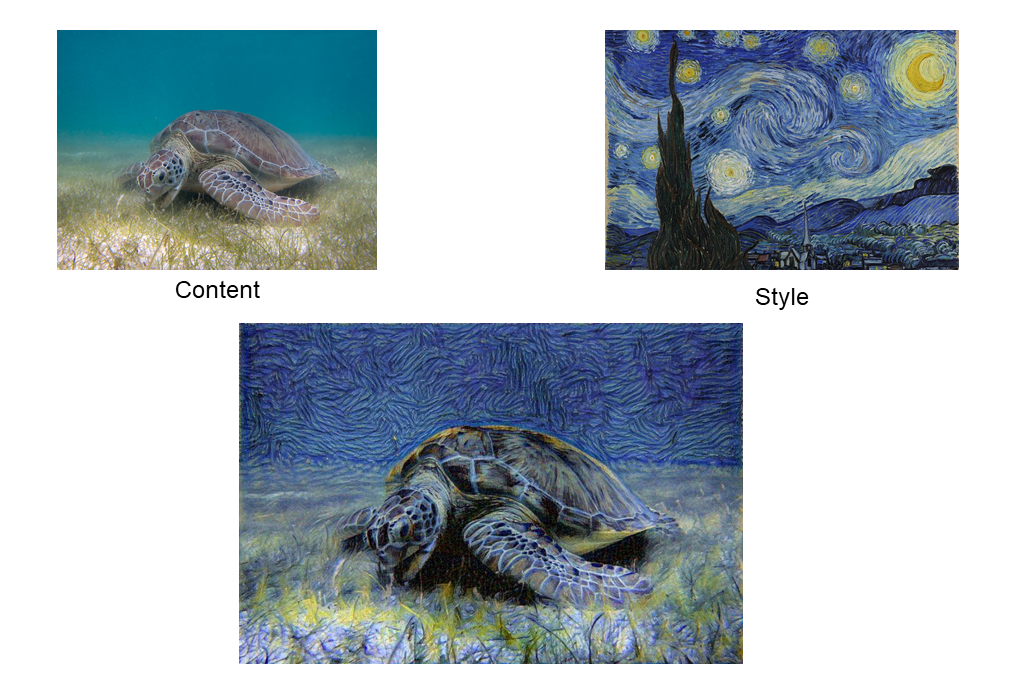
\includegraphics[width=\linewidth]{Ex_cropped.png}
	\caption{Příklad Paint Style Transfer. Vstupním obrázkem nesoucí obsah byla želva, stylem byla malba Starry Night. Výsledkem je obrázek želvy, jako by byla namalovaná ve stylu Starry Night.}
	\label{fig1}
	\end{figure}
	\par
	Jedním z prvních článků, věnující se této úloze za použití neuronových sítí, a zároveň článkem, z nějž vycházeli autoři tohoto textu je A Neural Algorithm of Artistic Style od Leona A. Gatyse et al. \footnote{https://arxiv.org/pdf/1508.06576.pdf} Gatys ve svém článku používal předtrénovanou síť VGG--19, v níž pozměnil max-pooling vrstvy za avg-pooling. Vstupem takovéto sítě pak byl obrázek, zpočátku bílý šum, který se během jednotlivých iterací aktualizoval na základě hodnot Loss funkce. Při tvorbě výstupního obrázku tedy nejsou aktualizovány parametry neuronové sítě, ale jednotlivé pixely toho obrázku a to tak, aby byla minimalizována hodnota Loss funkce. Označíme-li průběžně generovaný výstupní obrázek $\overrightarrow{x}$, \textit{content}  $\overrightarrow{p}$ a \textit{style}  $\overrightarrow{a}$, má Loss funkce $L_{total}$ tvar
	\begin{equation*}
		L_{total}(\overrightarrow{p}, \overrightarrow{a}, \overrightarrow{x}) = \alpha L_{content}(\overrightarrow{p}, \overrightarrow{x}) + \beta L_{style} (\overrightarrow{a}, \overrightarrow{x})
	\end{equation*}
	kde $L_{content}$ a $L_{style}$ jsou funkce počítající, jak se generovaný obrázek $\overrightarrow{x}$ liší obsahem od obsahového obrázku \textit{content} resp. stylem od stylového obrázku \textit{style} a $\alpha$ a $\beta$ jsou váhy těchto hodnot. V článku se používaly poměry $\alpha / \beta = 10^{-3}$ nebo $10^{-4}$.
	\par
	Dílčí Loss funkce $L_{content}$, měřící rozdíl obsahu mezi  $\overrightarrow{x}$ a  $\overrightarrow{p}$ porovnává aktivační mapy na $l$--té konvoluční vrstvě. Má-li tato vrstva $N_l$ filtrů a aktivační mapy mají $M_l$ pixelů, budou porovnávané matice $Q \in R^{N_l \times M_l}$. Jejich řádky budou představovat jednotlivé konvoluční filtry vrstvy a sloupce aktivační mapy těchto filtrů, převedené na vektor. Nyní, máme-li matice $F$ a $P$ obsahující tyto matice obrázků $\overrightarrow{x}$ a  $\overrightarrow{p}$, je $L_{content}$ spočtena jako
		\begin{equation*}
		L_{content} = \dfrac{1}{2} \sum_{i,j} (F_{ij} - P_{ij})^2
	\end{equation*}
	kde $i$ je index filtru a $j$ je index pixelu. V původním článku byla pro výpočet použita vrstva Conv4\_2.
	\par
	$L_{style}$, měřící rozdíl stylu mezi  $\overrightarrow{x}$ a  $\overrightarrow{a}$ se oproti $L_{content}$ nepočítá pouze nad jednou vrstvou ale nad několika. Je to z toho důvodu, že jinak hluboké vrstvy detekují jinak komplexní prvky stylu (např. mělčí vrstvy budou detekovat puze barvy, zatímco hlubší vrstvy mohou detekovat komplexnější entity jako tahy štětce) a pro kvalitní výsledek je podle Gatyse potřeba kombinace několika různě hlubokých vrstev. $L_{style}$ je počítána pomocí gram matice. Ta počítá korelaci mezi filtry a míru jejich aktivace na jedné vrstvě. To si lze představit na příkladu, kdy máme dva filtry, jeden detekující modrou barvu a druhý detekující spirály. Pokud by tyto filtry měly vysokou korelaci, znamenalo by to, že bude každá spirála v obrazu modrá. Samotná gram matice je vypočtena opět pomocí matice $Q$. Pro $l$--tou vrstvu tedy $Q \in R^{N_l \times M_l}$. $Q$ je poté vynásobena sebou samou v transponované formě a tedy výsledná gram matice $G \in R^{ N_l \times N_l}$.
	\begin{equation*}
		G = Q \times Q^T
	\end{equation*}
	V $l$--té vrstvě je pak odchylka stylů $\overrightarrow{x}$ s gram maticí $G^l$ a \textit{style} s gram maticí $A^l$ spočtena jako
	\begin{equation*}
		E_l = \frac{1}{4N_l^2M^2_l} \sum_{i,j}(G_{ij}^l - A_{ij}^l)^2
	\end{equation*}
	Napříč všemi vrstvami je poté $L_{style}$ spočtena jako
		\begin{equation*}
		L_{syle} = \sum_{l=0}^{L} w_l E_l
	\end{equation*}
	kde $E_l$ jsou dílčí chyby z různých vrstev a $w_l$ jsou váhy těchto chyb. Gatys používal rovnoměrně rozdělené váhy, které v součtu dají hodnotu $1$. V článku se používají chyby z vrstev Conv1\_1, Conv2\_1, Conv3\_1, Conv4\_1 a Conv5\_1.
	\\
	Na obrázku \ref{VGG} je vyobrazena používaná síť VGG--19 spolu s místy, z nichž se počítá chyba.
	\begin{figure}[h]
	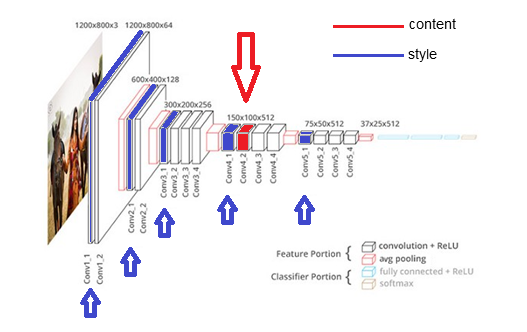
\includegraphics[width=\linewidth]{VGG.png}
	\caption{Znázornění použité architektury. Jsou zde také vyznačena místa, z nichž jsou počítány chyby. Původní obrázek převzat z https://towardsdatascience.com/art-with-ai-turning-photographs-into-artwork-with-neural-style-transfer-8144ece44bed}
	\label{VGG}
\end{figure}
	
\section*{Datová sada}
	Naše datová sada se dělí do dvou sekcí. První je sekce stylových obrázků, obsahující díla známých autorů, napříč styly (například Wassily Kandinsky -- Composition VII, nebo Vincent van Gogh -- Starry Night), které byly vybrány tak, aby zastupovaly co možná nejširší záběr výtvarného projevu. V této části datové sady se nalézá 6 děl. 
	\par
	
	Druhá část sady obsahuje 5 "content" obrázků. Tentokrát se jedná o fotografie různých objektů. Opět jsme se snažili o co možná nejpestřejší výběr. V sadě se tak nalézá například hromada kovových součástí strojů, nebo fotografie rozvětveného stromu.
	\par
	Celá datová sada je dostupná na GitHubu tohoto projektu\footnote{https://github.com/Zjelin/paint\_style\_transfer}. Zde jsou také uvedené zdroje, z nichž bylo čerpáno. 

	\section*{Experimenty}
	V rámci experimentů s naší implementací jsme se rozhodli porovnat rychlost konvergence různých optimalizátorů, vyzkoušet vliv výběru odlišných vrstev pro výpočet $L_{style}$ a \textbf{vyzkoušet vliv změny počátečního obrázku z bílého šumu na content obrázek}. Hodnoty $\alpha$ a $\beta$ byly nastaveny na $\alpha = 10^{-1}$ $\beta = 10^6$ a tedy poměr $\alpha / \beta = 10^{-7} $. Tento poměr byl vybrán z toho důvodu, že produkoval $L_{total}$ hodnoty blízko 0 a dle autorů na něm šly  dobře pozorovat rozdíly v chování během jednotlivých experimentů. V rámci experimentů používáme 3 \textit{style} a 3 \textit{content} obrázky, které jsou vyobrazeny na obrázku \ref{UsedFigs}. Tyto obrázky pužíváme v \textit{content-style} párech \textit{machinery-sea}, \textit{tree-wave} a \textit{barcelona-figure}.
	\begin{figure}[h]
		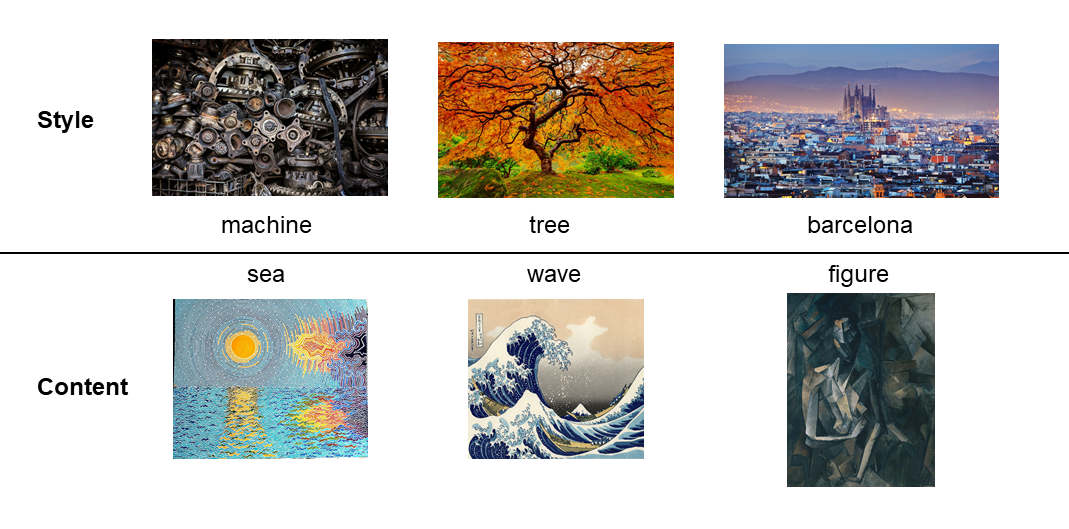
\includegraphics[width=\linewidth]{figs.png}
		\caption{Obrázky použité v rámci experimentů. Jejich zdroje jsou uvedeny na gitu projektu.}
		\label{UsedFigs}
	\end{figure}
	
	
	\subsection*{Test optimalizátorů}
	V rámci prvotní implementace, která byla vytvořena pomocí frameworku TensorFlow jsme zkoušeli téměř všechny její základní optimalizátory\footnote{https://www.tensorflow.org/api\_docs/python/tf/keras/optimizers} z hlediska rychlosti konvergence a shledali jsme, že nejrychleji konverguje optimalizátor Adam. Když jsme však chtěli použít optimalizátor LBFGS, avšak v TensorFlow se nám jej nedařilo implementovat. To byl hlavní důvod migrace naší implementace do frameworku PyTorch.
	\par
	V rámci experimentu jsme porovnávali optimalizátory Adam a LBFGS. Learning rate Adama byl nastaven na $0,01$, pro LBFGS byl nastaven na $0,8$. Výsledky experimentů zobrazují grafy na obrázku \ref{exp1G}.
	
	\begin{figure}[h]
		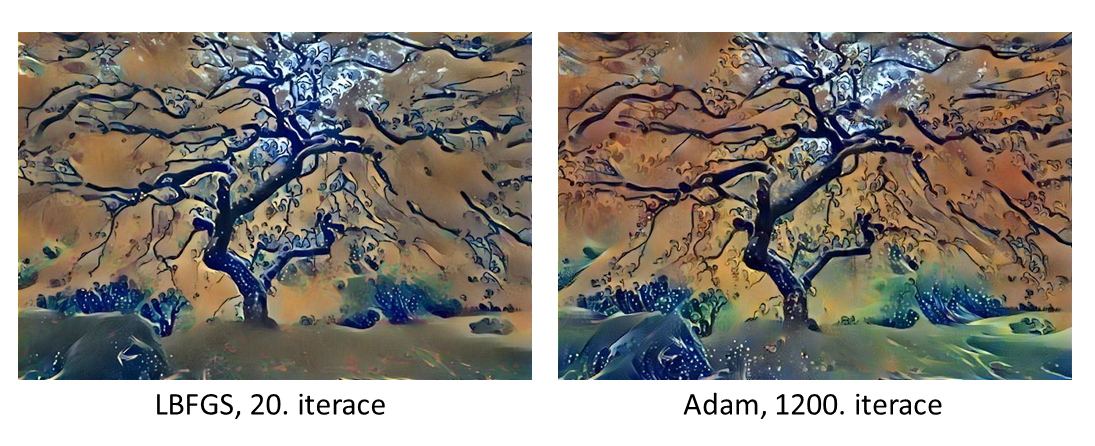
\includegraphics[width=\linewidth]{LBFGS_ADAM_iterace.png}
		\caption{Porovnání výsledků optimalizátorů. }
		\label{Exp1O}
	\end{figure}
	
	

	Z grafů lze vyčíst, že rychlost konvergence při použití optimalizátoru LBFGS je řádově rychlejší, než při použití Adama. Už po 20. iteraci dokázal LBFGS vygenerovat přijatelný výsledek, kdežto Adamovi trvalo vygenerování vizuálně zajímavějšího výsledku okolo 1000 iterací, viz \ref{Exp1O}.

	 Dalším zajímavým jevem je, že v případě optimalizátoru Adam občas docházelo k nenadálému nárůstu Loss hodnoty. Pro tento úkaz nemají autoři vysvětlení.
	
	\subsection*{Test stylových vrstev}
	Dalším experimentem, který byl vykonán bylo testování, nakolik závisí rychlost konvergence Loss funkce a vizuální kvalita výstupu na výběru vrstev, na nichž se počítá $L_{style}$. Při experimentu byl ponechán počet iterací výpočtu. Style loss byl pro účely experimentu počínán kromě původních vrstev, navrhovaných Gatysem počítán z Conv1\_1, Conv1\_2, Conv2\_1, Conv2\_2, a Conv3\_1.
	Jejich srovnání je z hlediska konvergence Loss funkce zobrazeno na obrázku \ref{Exp2_G} a porovnání kvality výstupu je na obrázku \ref{Exp2_O}. Pro porovnání byly opět použity stejné tři dvojice obrázků.
	\par
	Z grafu vývoje Loss funkce obrazů, jejichž styl byl generován z mělčích vrstev, lze vypozorovat, že ve všech případech skončila hodnota Loss po poslední iteraci níž než v obrazech generovaných za pomocí původních vrstev. Dle autorů by to mohlo být způsobeno jednoduššími entitami, které jsou v těchto vrstvách detekovány. Dále se u vývoje Loss hodnoty pro nově vybrané vrstvy opět objevují nenadálé výkyvy. 
	\par
	Z vizuálního hlediska mají obrazy generované mělčími vrstvami barevně výraznější schéma, které přejali ze stylového obrázku. Při použití mělčích vrstev se propaguje spíše barva (low-level features), než komplexnější vzorce. Např. na dvojici \textit{tree-wave} si lze všimnout, že při použití originálních vrstev se projevily vzorce vln ve větší míře (porovnejme levé spodní části obrázků). 
	 
	\subsection*{Test počátečního generovaného obrázku}
	Výsledný obrázek, který je napříč iteracemi výpočtu upravován tak, aby minimalizoval Loss hodnotu je v původním článku od Gatyse inicializován na bílý šum. Během optimalizace se pak snižuje jak Content Loss, tak Style Loss, když z náhodného šumu vzniká výsledný obrázek. Naše řešení však za výchozí výstup používá Content obrázek. Tato idea na změnu výchozího stavu byla přejata ze serveru medium.com\footnote{https://medium.com/tensorflow/neural\-style\-transfer\-creating\-art\-with\-deep\-learning\-using\-tf\-keras\-and\-eager\-execution\-7d541ac31398}, podle nějž byla tvořena původní implementace pomocí frameworku TensorFlow. V tomto experimentu si klademe za cíl určit, zda má tato změna vliv na kvalitu výstupu/rychlost konvergence.
	\par
	Pro generování výsledků s použitím bílého šumu byl použit optimalizátor LBFGS při 100 iteracích. Příklad porovnání výstupů, je na obr. \ref{Noise}. Z výsledků lze usoudit, že inicializace s Content obrázkem je výhodná, neboť konverguje rychleji. Toto je podle autorů dáno tím, že content je již ve výstupu přítomen a není tak třeba jej tam zanášet (tj. snižovat Content Loss hodnotu).
	
		\begin{figure}[h]
		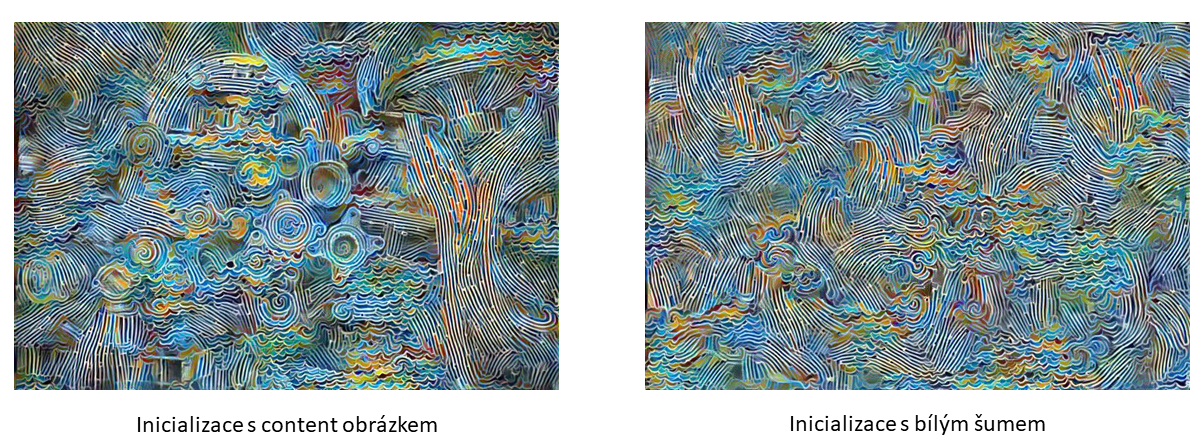
\includegraphics[width=\linewidth]{ContentNoise.png}
		\caption{Porovnání výsledků s různými inicializačními obrázky. }
		\label{Noise}
	\end{figure}
	
	\section*{Závěr}
	V tomto projektu jsme realizovali řešení úlohy Paint Style Transfer navržené Gatysem. Implementace byla řešena v jazyce Python3, s využitím frameworku PyTorch.
	\par
	V rámci experimentů jsme porovnali efektivitu optimalizátorů, z nichž nejlépe vyšel LBFGS. Dále jsme navrhli alternativní volbu stylových vrstev, kde jsme vybrali vrstvy mělčí. Alternativní vrstvy dosahovaly rozdílných vizuálních výsledků. Nelze jednoznačně určit, která volba je vhodnější, neboť ani jedna série výsledků není signifikantně horší a vkus je subjektivní. Prokázali jsme, že inicializace výstupního obrázku je výhodnější za použití Content obrázku, namísto bílého šumu používaného Gatysem v původním článku.
	

		\begin{figure*}[t]
		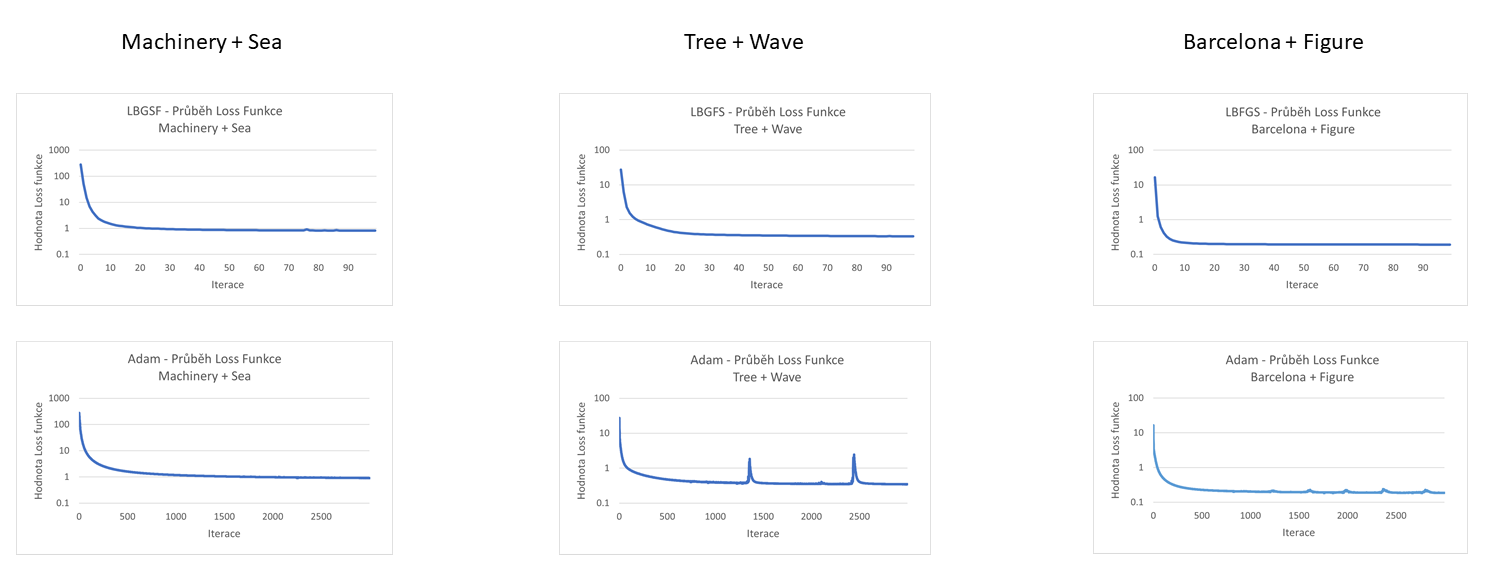
\includegraphics[width=18cm]{Ex1G_lez.png}
		\caption{Průběh Loss funkce při použití různých optimalizátorů. První řádek reprezentuje použití optimalizátoru LBFGS, druhý použití Adama.}
		\label{exp1G}
	\end{figure*}
	
	
	\begin{figure*}[t]
		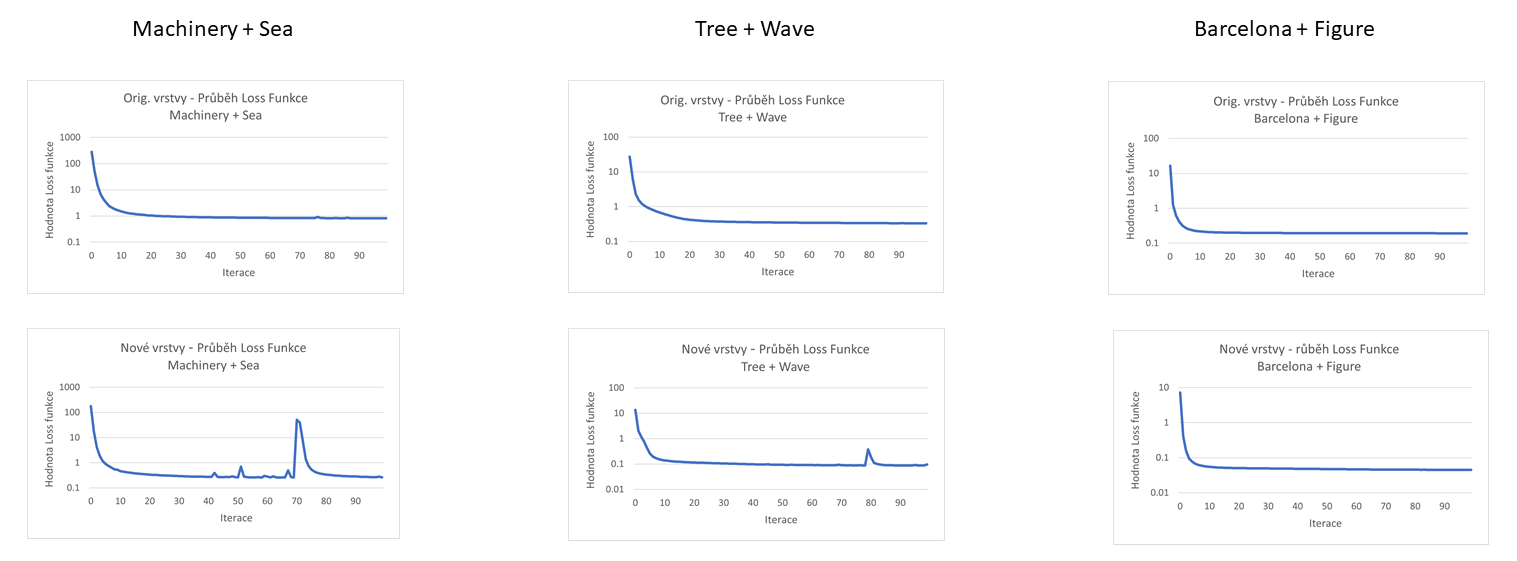
\includegraphics[width=18cm]{Ex2G_lez.png}
		\caption{Průběh Loss funkce při počítání $L_{style}$z různých vrstev. Nahoře Conv1\_1, Conv2\_1, Conv3\_1, Conv4\_1 a Conv5\_1. Dole Conv1\_1, Conv1\_2, Conv2\_1, Conv2\_2, a Conv3\_1.}
		\label{Exp2_G}
	\end{figure*}

	
\begin{figure*}[h]
	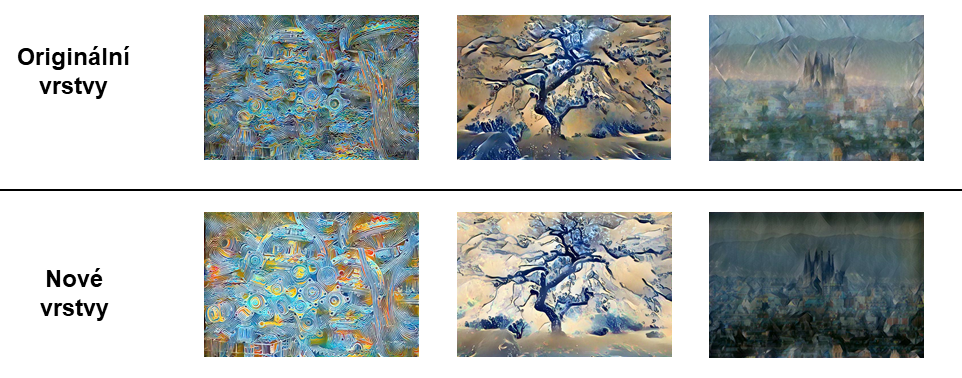
\includegraphics[width=\linewidth]{Ex2O_lez.png}
	\centering
	\caption{Obrázky generované pomocí původních vrstev (nahoře) a pomocí nově zvolených stylových vrstev (dole).}
	\label{Exp2_O}
\end{figure*}

\end{document}
